\subsection{OSI - Data Link Layer}

	\par{The main purpose of the data link layer is to arbitrate access to the physical layer and turn the raw bit stream of data into a structured communications channel with the goal of transferring data between nodes attached to the same physical cable. There are several services provided by the DDL, the main ones being: \ita{Media Access Control (MAC addressing) , Error detection and/or correction, Framing}}


	\subsubsection{Framing}

		\par{Frames are essentially fenced packets, which signal to the next layer the significant part of the data , i.e the \ita{payload} and often whether that data was corrupted via some sort of error code or \ita{checksum}. The DLL add the final tail and header to the payload and is therefore responsible for the last bit of data \ita{encapsulation}}

		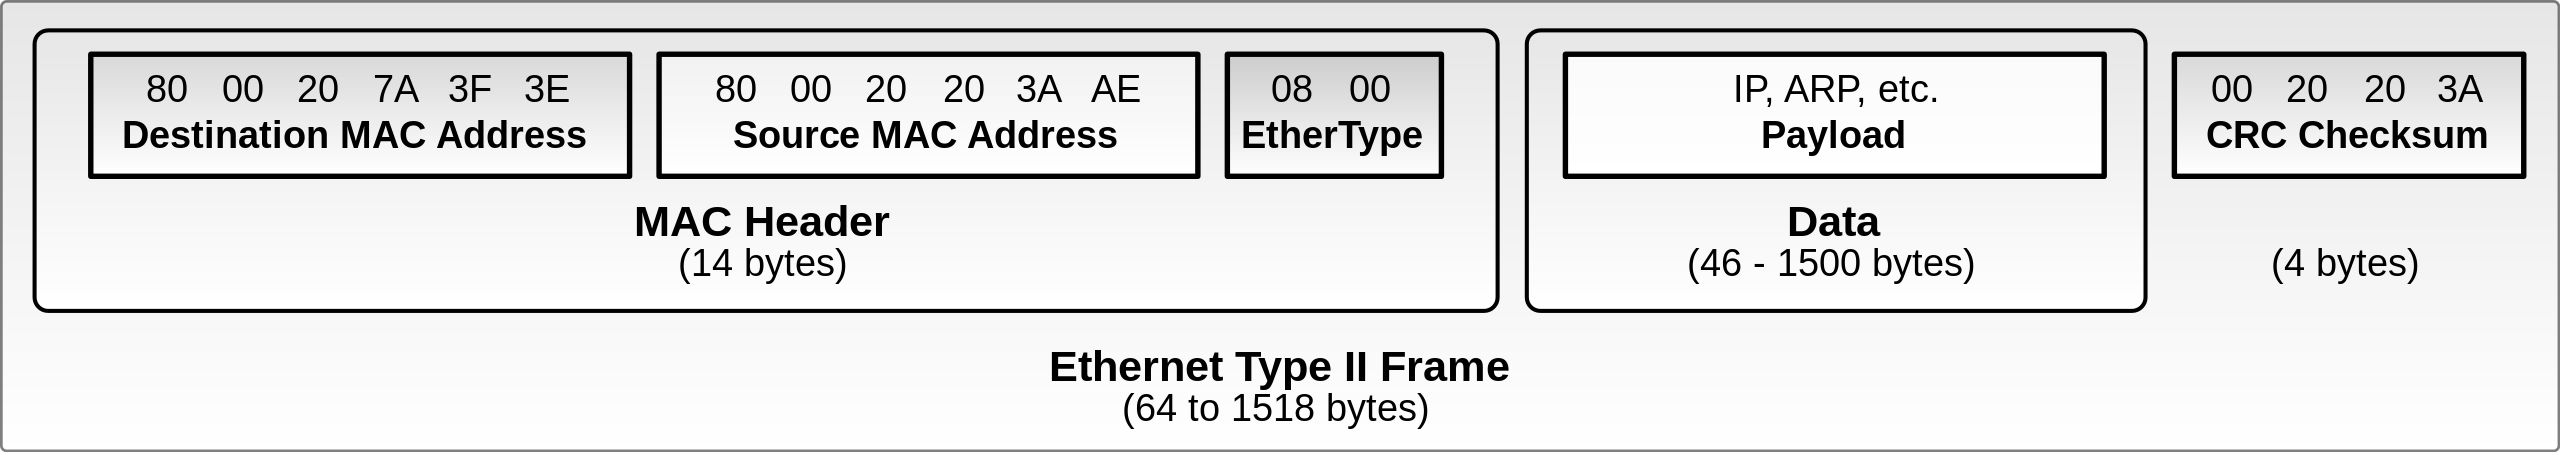
\includegraphics[width=0.7\textwidth]{frame}


	\subsubsection{Error Detection \& Correction}

		\par{Though rare in wired systems, it is quite common for noise to cause bit errors in the data being transmitted. If the DLL implements error detection then it must add a \ita{error detection code} as an header of the frame, the simplest one being the \ita{parity code}. When the receiver gets the packet it uses the same function/rule to recalculate the code, if it doesn't match the frame is either discarded or corrected}

		\defn{Parity Code}{an error detection code which is able to detect single bit errors. It works by adding all the bits, and checking the parity of their sum}

		\defn{Checksum}{works similarly to the parity code, but is able to handle some multiple bit errors by using a 16-bit one's complement checksum}

		\defn{Cyclic Redundancy Code}{a more advanced algorithm, commonly used in the DDL which can check if the bits are out of order. It relies on the remainder of a polynomial division of the data being sent}


	\subsubsection{MAC}

		\par{MAC is needed to determine which machine gets access to the channel when multiple hosts try to access it simultaneously. Because if that happens then the signals are said to \ita{collide} and will overlap, resulting in an unreadable/garbage message.}

		\defn{Contention-Based MAC}{a system is contention-based if multiple hosts share a channel in a way that can lead to collisions}

		\par{CB MAC deals with collision in one of two ways:}

			\begin{enumerate}
				\item \textbf{ALOHA} is the simplest protocol developed at the University of Hawaii in 1970. It tries to transmit whenever data is available, and if a collision occurs the frames are destroyed and the node will wait for a random amount of time before retransmitting, repeating until successful.

				\item \textbf{CSMA} listens to the channel before sending, if it hears no traffic then it starts transmitting. Note however, that if the message takes time to reach the node , i.e. if there's a high \ita{propagation delay} then there is an increased probability of a collision occurring mid-transit, an improved algorithm is \textbf{CSMA/CD} where the sending node keeps listening even during sending, if a collision occurs then both stations cease transmission immediately. This is an improvement because even though the frames are still corrupted, it saves time and bandwidth by reducing the time the channel is blocked due to collision.
				\mymarginpar{The back-of interval between retransmissions is also random, but should increase with the number of collisions to reduce congestion}
			\end{enumerate}

	




	\subsubsection{Summary}
		\begin{itemize}
			\item\textbf{PDU : } series of bits - \ita{frame}
			\item\textbf{Function : } Physical addressing , Framing, Error Detection
			\item Last encapsulation of data step ; adds an error detection code and some other meta data for framing in the trail of the packet
			\item Simpler error detection codes rely on summing up the bits of data and either checking their parity or sum
			\item Contention-Based MAC handle collisions by listening to the channel before sending the data and/or during
		\end{itemize}
